% chktex-file 2
% chktex-file 8
% chktex-file 12
% chktex-file 13
% chktex-file 18
% chktex-file 24
% chktex-file 26
% chktex-file 35
% chktex-file 44
% chktex-file 45

\documentclass[]{article}
\usepackage[utf8]{inputenc}
\usepackage[english]{babel}

% imports %%%%%%%%%%%%%%%%%%%%%%%%%%%%%%%%%%%%%%%%%%%%%%%%%%%%%%

\usepackage[]{csvsimple}
\usepackage[]{afterpage}
\usepackage[]{float}

\usepackage{ragged2e}
\usepackage[left=25mm, right=25mm, top=15mm]{geometry}
\geometry{a4paper}
\usepackage{graphicx}
\usepackage{booktabs}
\usepackage{paralist}
\usepackage{subfig} 
\usepackage{fancyhdr}
\usepackage{amsmath}
\usepackage{amssymb}
\usepackage{amsfonts}
\usepackage{amsthm}
\usepackage{mathtools}
\usepackage{enumitem}
\usepackage{titlesec}
\usepackage{braket}
\usepackage{gensymb}
\usepackage{url}
\usepackage{hyperref}
\usepackage{csquotes}
\usepackage{multicol}
\usepackage{graphicx}
\usepackage{wrapfig}
\usepackage{babel}
\usepackage{caption}
\captionsetup{font=small}
\pagestyle{fancy}
\renewcommand{\headrulewidth}{0pt}
\lhead{}\chead{}\rhead{}
\lfoot{}\cfoot{\thepage}\rfoot{}
\usepackage{sectsty}
\usepackage[nottoc,notlof,notlot]{tocbibind}
\usepackage[titles,subfigure]{tocloft}
\renewcommand{\cftsecfont}{\rmfamily\mdseries\upshape}
\renewcommand{\cftsecpagefont}{\rmfamily\mdseries\upshape}

\let\oldsection\section% Store \section
\renewcommand{\section}{% Update \section
	\renewcommand{\theequation}{\thesection.\arabic{equation}}% Update equation number
	\oldsection}% Regular \section
\let\oldsubsection\subsection% Store \subsection
\renewcommand{\subsection}{% Update \subsection
	\renewcommand{\theequation}{\thesubsection.\arabic{equation}}% Update equation number
	\oldsubsection}% Regular \subsection

\newcommand{\abs}[1]{\left\lvert#1\right\rvert}
\newcommand{\norm}[1]{\left\lVert#1\right\rVert}

\newcommand{\g}{\text{g}}
\newcommand{\m}{\text{m}}
\newcommand{\cm}{\text{cm}}
\newcommand{\mm}{\text{mm}}
\newcommand{\s}{\text{s}}
\newcommand{\N}{\text{N}}
\newcommand{\Hz}{\text{Hz}}

\newcommand{\virgolette}[1]{``\text{#1}"}
\newcommand{\tildetext}{\raise.17ex\hbox{$\scriptstyle\mathtt{\sim}$}}

\renewcommand{\arraystretch}{1.2}

\addto\captionsenglish{\renewcommand{\figurename}{Fig.}}
\addto\captionsenglish{\renewcommand{\tablename}{Tab.}}

\DeclareCaptionLabelFormat{andtable}{#1~#2  \&  \tablename~\thetable}

%%%%%%%%%%%%%%%%%%%%%%%%%%%%%%%%%%%%%%%%%%%%%%%%%%%%%%%%%%%%%%%

%opening
\title{%
    \Huge Misura indiretta della velocità della luce \\
    \Large Laboratorio di Ottica, Elettronica e Fisica Moderna \\ C.d.L. in Fisica, a.a. 2023-2024 \\ Università degli Studi di Milano}
\author{\LARGE Lucrezia Bioni, Leonardo Cerasi, Giulia Federica Bianca Coppi \\ Matricole: 13655A, 11410A, 11823A}
\date{19 ottobre 2023}

\begin{document}

    \maketitle

    \section{Introduzione}

    Lo scopo di questa esperienza è la misurazione della velocità della luce utilizzando 
    il metodo di Focault. Questa grandezza, infatti, svolge un ruolo cruciale come costante 
    fisica universale e la sua determinazione è stata di fondamentale importanza per la definizione 
    delle unità di misura nel Sistema Internazionale. \\
    Il valore che, attualmente, è universalmente accettato come misura più precisa della velocità della luce è $\bar{c} = 299792456.2 \,\text{m/s}$.

    \subsection{Metodo}
    
    La determinazione della velocità della luce viene effettuata utilizzando il metodo di Focault: 
    viene diretto un fascio luminoso, proveniente da una sorgente, verso uno specchio rotante che ne causa la riflessione con uno spostamento angolare.\\
    Il raggio di luce, dopo aver colpito lo specchio rotante, viene riflesso nella direzione opposta lungo la stessa traiettoria che aveva compiuto nel viaggio di andata. Poiché lo specchio è in rotazione, la posizione in cui il raggio colpisce lo specchio è in costante cambiamento: questo causa uno spostamento angolare tra il punto di arrivo del raggio riflesso e la posizione iniziale - misurata con specchio fermo.\\
    Misurando con precisione la posizione iniziale $ \delta _i $ dello spot luminoso - con specchio fermo - e la finale  $ \delta _f $ - con specchio in movimento - si riesce a dedurre lo spostamento angolare $ \Delta \delta = \delta_f - \delta_i $: questo rende possibile determinare la velocità della luce:
    \begin{equation}
        \label{eqn-c}
        c=4 f_2 D^2 \frac{(\omega -\omega_0)}{(D+a-f_2)\Delta \delta }
    \end{equation}
    dove $ c $ è la velocità della luce, $ f_2 $ è la lunghezza focale della seconda lente posta nell'apparato, $ D $ è la lunghezza del percorso compiuto dal fascio luminoso, $ \omega_0 $ e $ \omega $ sono rispettivamente la velocità angolare iniziale e finale dello specchio rotante, $ a $ è la distanza tra la seconda lente dell'apparato e lo specchio rotante e $ \Delta\delta$ è lo spostamento dell'immagine nel punto di osservazione, quando la velocità angolare dello specchio rotante passa da $ \omega_0 $ a $ \omega $.
    % da modificare
    Per uno schema dell'apparato sperimentale si veda la Fig. \ref{schema}.
    \begin{figure}[h]
        \centering
        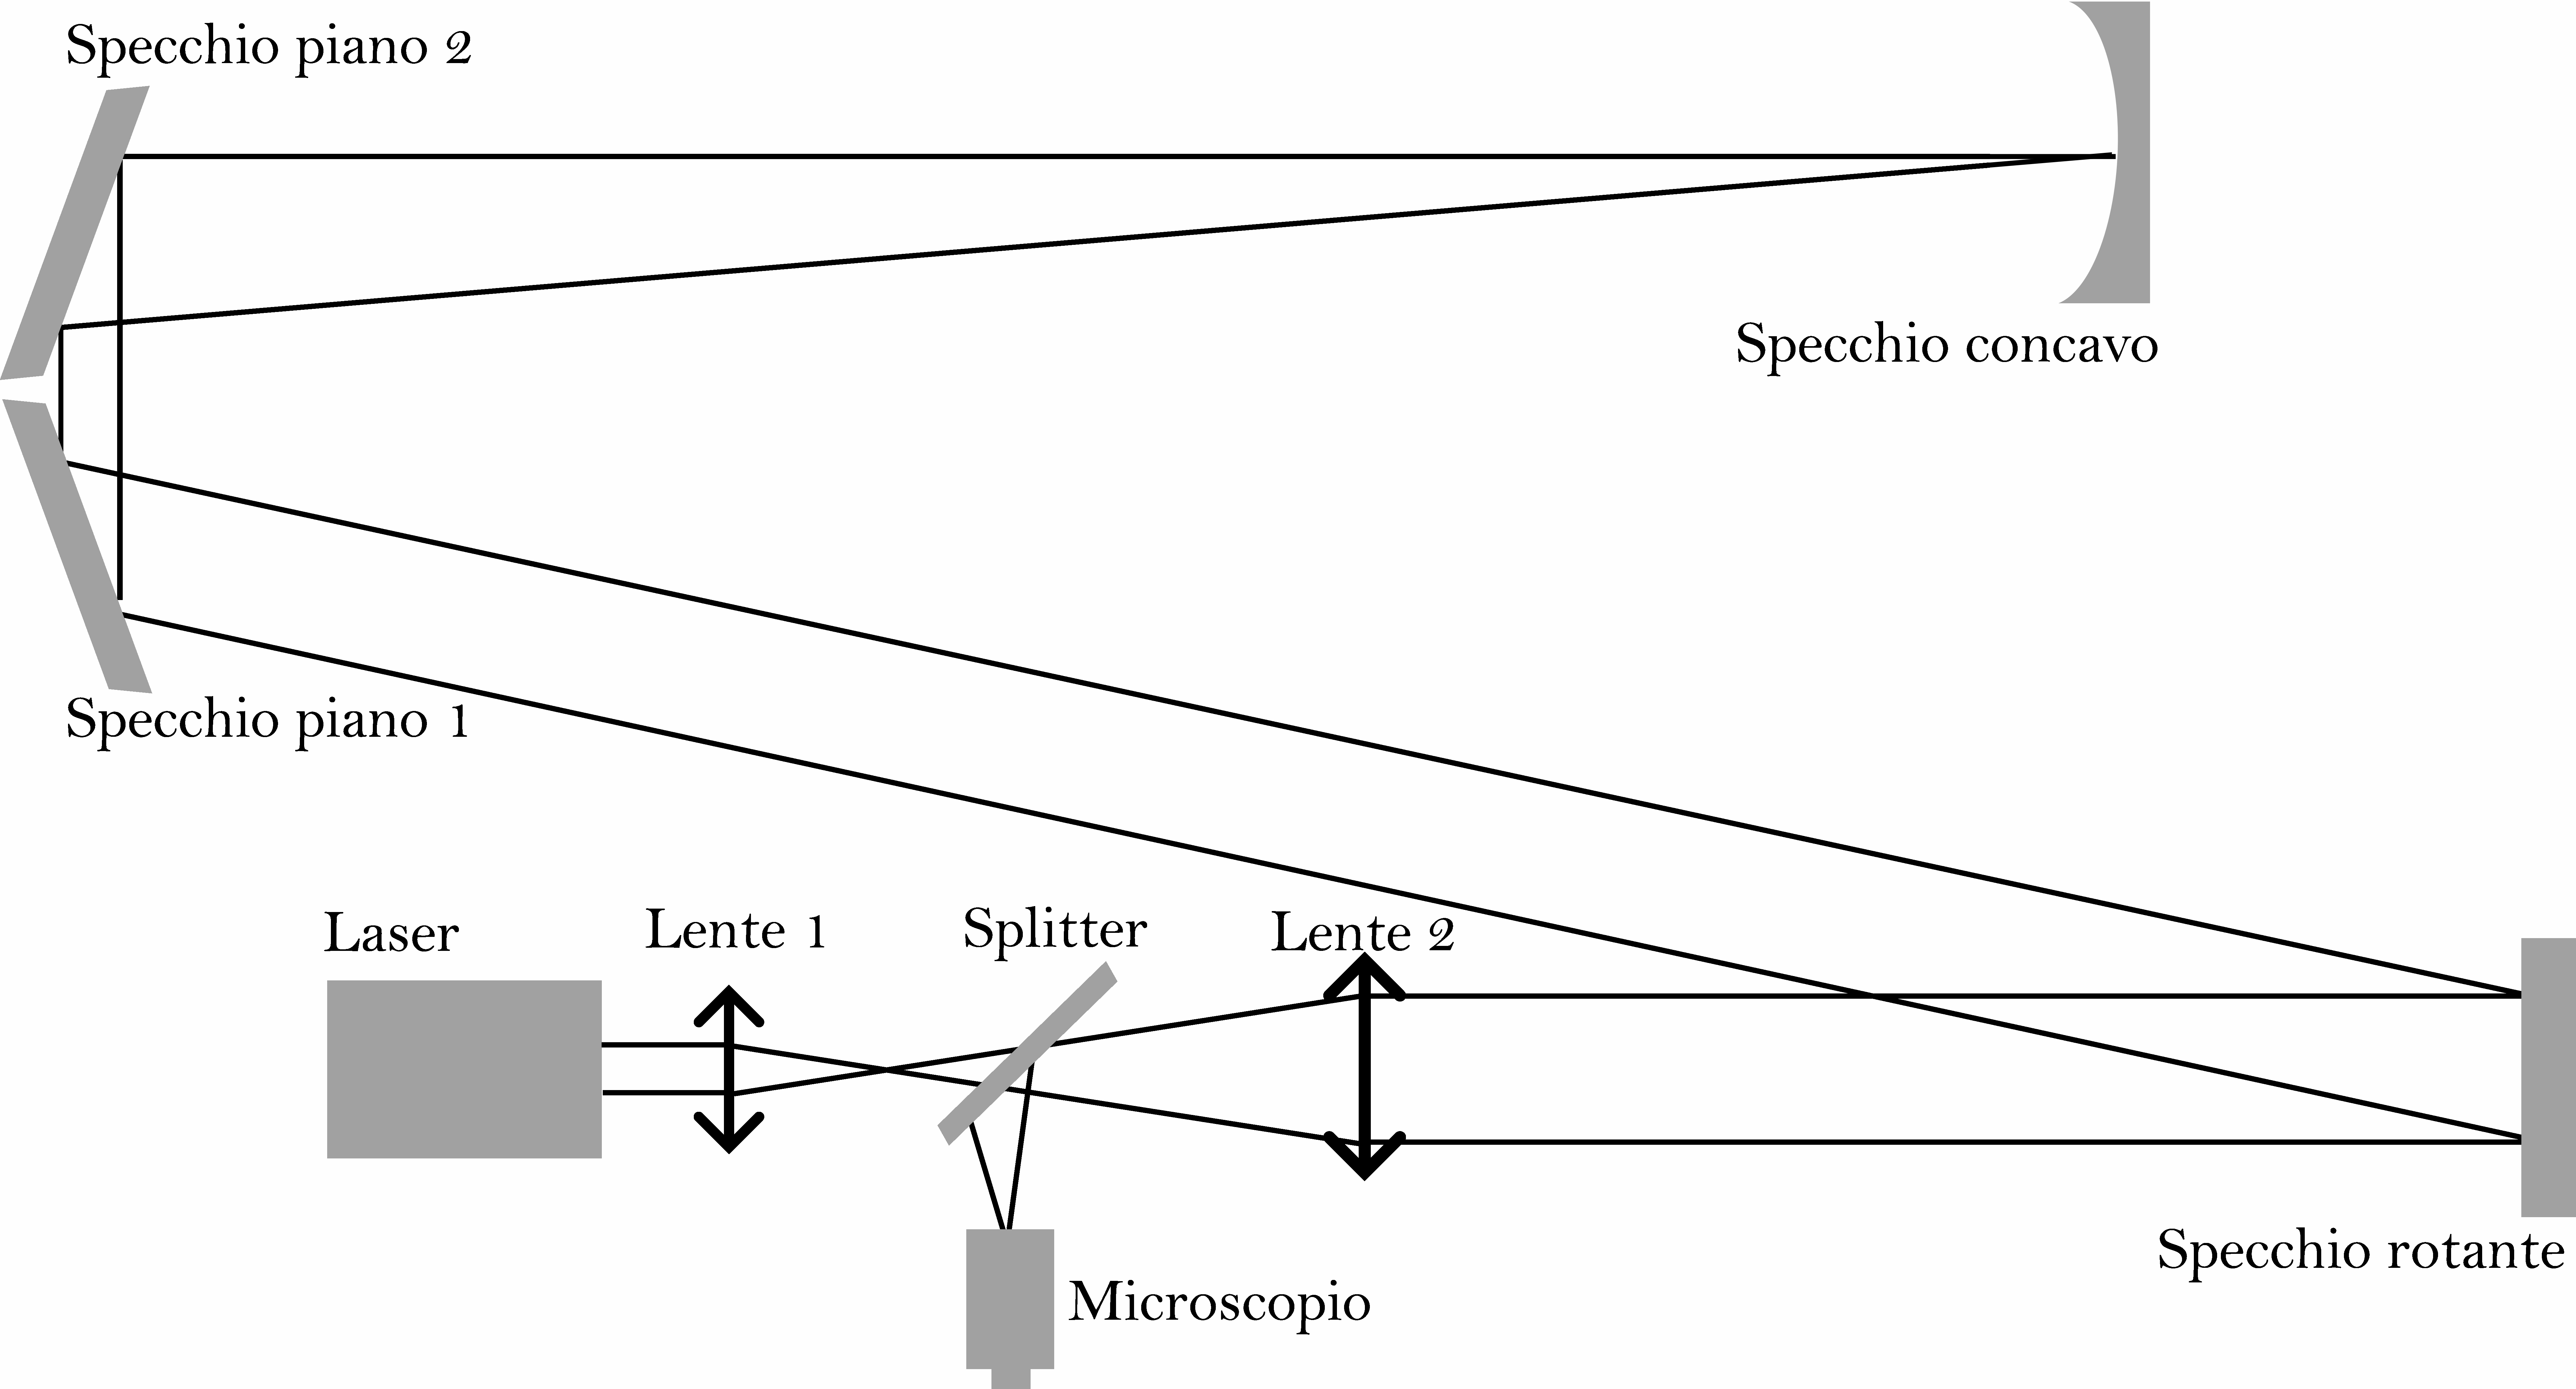
\includegraphics[width=0.70\textwidth]{disegnetto-apparato.png}
        \caption{Schema dell'apparato sperimentale.}
        \label{schema}
    \end{figure}

    \section{Misure}
    
    Si è inizialmente misurata la distanza $D$ tra lo specchio rotante e lo specchio concavo. La distanza $D$ è stata misurata mediante un metro di risoluzione $ 0.01 \, \text{m} $, la quale è stata attribuita come incertezza al valore della misura:
    \begin{equation}
        \label{equation-for-D}
        D = (13.28 \pm 0.01) \, \text{m}
    \end{equation} \\
    Si è poi misurata la distanza $a$ tra la seconda lente dell'apparato e lo specchio rotante. La misura è stata effettuata attraverso un metro di risoluzione $ 0.001 \, \text{m} $, che è stata attribuita come incertezza di $a$:
    \begin{equation}
        \label{equation for a}
        a = (0.474 \pm 0.001) \, \text{m}
    \end{equation}

    Dopo aver avviato lo specchio rotante in senso orario a una frequenza di rotazione $ \nu_0 $ nell'intervallo $[10,20] \, \text{Hz}$, si è misurata, mediante micrometro di risoluzione $ 0.00001 \text{m} $, la posizione dello spot luminoso $\delta_0$ visibile attraverso un microscopio. Si è poi portato lo specchio in un intorno della frequenza massima di rotazione $ \nu $ e si è misurata, sempre mediante micrometro, la nuova posizione dello spot luminoso $\delta$. Tale set di misure è stato ripetuto per $30$ volte. I dati rilevati sono riportati nella Tab. \ref{CW_min_max-delta-omega}. \\
    Si sono prese le medesime misure di posizione, a frequenza minima e a frequenza massima, facendo ruotare lo specchio in senso antiorario. I dati rilevati sono riportati nella Tab. \ref{CCW_min_max-delta-omega}. \\
    Si sono poi effettuate misure di posizione dello spot luminoso portando lo specchio dalla frequenza massima di rotazione in senso orario $\nu_0$ alla frequenza massima di rotazione in senso antiorario $\nu$. I dati rilevati sono riportati nella Tab. \ref{CW_CCW-delta-omega}. \\
    Infine, si sono rilevate misure di posizione dello spot luminoso con lo specchio a frequenza minima di rotazione ($[10,20] \, \text{Hz}$) e a frequenze intermedie, sia in senso orario (i dati sono riportati nella Tab. \ref{CW_min_mid-delta-omega}) sia in senso antiorario (i dati sono riportati nella Tab. \ref{CCW_min_mid-deta-omega}).

    \section{Analisi Dati}

    \subsection{Elaborazione Dati}

    A partire dalle coppie di misurazioni della frequenza di rotazione dello specchio $ \nu $ e della deviazione dello spot luminoso del laser $ \delta $ per ciascuna configurazione, sono state calcolate la velocità angolare $ \omega = 2\pi\nu $ e le rispettive variazioni $ \Delta\omega $ e $ \Delta\delta $ al variare della frequenza: i dati così elaborati sono riportati in Tabb. \ref{CW_min_max-c}, \ref{CCW_min_max-c}, \ref{CW_CCW-c}, \ref{CW_min_mid-c}, \ref{CCW_min_mid-c}. \\
    Una volta ottenuta ciascuna coppia $ \left(\Delta\omega,\Delta\delta\right) $, sono stati ricavati i valori della velocità della luce $c$ tramite l'equazione \ref{eqn-c}, i quali vengono presentati nelle Tabb. \ref{CW_min_max-c}, \ref{CCW_min_max-c}, \ref{CW_CCW-c}, \ref{CW_min_mid-c}, \ref{CCW_min_mid-c}. Attraverso la meda aritmetica dei valori di $c$ così ottenuti, si è estrapolato un valore della velocità della luce per ciascuna configurazione (si veda Tab. \ref{c-values}).

    \subsection {Stima degli errori}

    L'errore sulla stima del valore di $ c $, $ \sigma_{c,tot} $, è frutto di due componenti, una statistica $\sigma_{c,stat}$ e una sistematica $\sigma_{c,sist}$:
    \begin{equation}
        \label{sigma_tot}
        \sigma_{c,tot} = \sqrt{ {\sigma_{c,stat}} ^2 + {\sigma_{c,sist}} ^2 } 
    \end{equation}
    La componente statistica viene determinata attraverso la deviazione standard della media dei valori ottenuti per $c$ per ogni set di misure di $ \Delta \omega $ e $ \Delta \delta $. \\
    La componente sistematica viene determinata attraverso la propagazione degli errori sulle misure delle grandezze $D$ e $a$ nella formula per la determinazione della velocità della luce \ref{eqn-c}. In tale procedimento si considerano le grandezze  $\omega$ e $\delta$ come prive di errore, poiché questo è già stato considerato nella componente statistica dell'errore:
    \begin{equation}
        \label{sigma-sist}
        \sigma_{c,sist} = \sqrt{ \left(\frac{\partial c}{\partial D}\right)^2 \, \sigma_D ^2 + \left(\frac{\partial c}{\partial a}\right)^2 \, \sigma_a ^2 } 
    \end{equation}
    dove:
    \begin{equation}
        \label{eqn-propD}
        \frac{\partial c}{\partial D} = \frac{4\Delta \omega}{\Delta \delta} \frac{D f_2 \left(2a + D -2f_2\right)}{\left(a + D -f_2\right)^2}
    \end{equation}

    \begin{equation}
        \label{eqn-propa}
        \frac{\partial c}{\partial a} = -\frac{4\Delta \omega}{\Delta \delta} \frac{D^2 f_2}{\left(a + D -f_2\right)^2}
    \end{equation}
    Per ciascuna configurazione, si è valutata la componente sistematica dell'errore sul valor medio della velocità della luce: come valori di $\Delta\omega$ e $\Delta\delta$ sono stati utilizzati i corrispondenti valori medi per ciascun set di dati.
    
    \subsection{Confronto}

    Per confrontare i valori della velocità della luce ottenuti per ciascuna configurazione con il valore aspettato $\bar{c} = 299792456.2 \,\text{m/s}$, si è utilizzato un test di Student a due code, con, a seconda della configurazione, gradi di libertà pari a $29$ o $14$, ottenuti dalla differenza tra il numero totale di misure effettuate ($30$ o $15$) e il numero di variabili statistiche estratte da queste ($1$). \\
    I valori di $c$ elaborati per ciascuna configurazione con i rispettivi errori sono riportati nella seguente tabella:
    
    \begin{table}[H]
        \centering
        \begin{tabular}{||c|c|c|c|c|c||}
            \hline
            Configurazione & $c \, [10^8 \,\text{m/s}]$ & $\sigma_{c,stat} \,[10^8 \,\text{m/s}]$ & $\sigma_{c,sist} \,[10^8 \,\text{m/s}]$ & $\sigma_{c,tot} \,[10^8 \,\text{m/s}]$ & Compatibilità \\
            \hline\hline
            CW-min-max & $3.044$ & $0.025$ & $0.002$ & $0.025$ & $6.90\%$ \\\hline
            CCW-min-max & $2.972$ & $0.021$ & $0.002$ & $0.021$ & $23.66\%$ \\\hline
            CW-CCW & $2.980$ & $0.012$ & $0.002$ & $0.012$ & $15.40\%$ \\\hline
            CW-min-mid & $2.983$ & $0.029$ & $0.002$ & $0.029$ & $60.90\%$ \\\hline
            CCW-min-mid & $2.978$ & $0.022$ & $0.002$ & $0.022$ & $37.16\%$ \\\hline
        \end{tabular}
        \caption{Valori di $c$ e relativi errori per ciascuna configurazione.}
        \label{c-values}
    \end{table}

    Dal test effettuato emerge che i valori di $c$ superano tutti la soglia minima di compatibilità stabilita al $5\%$. \\
    Sempre mediante test di Student si è eseguito un confronto tra le varie medie ottenute per ciascuna configurazione:

    \begin{table}[H]
        \centering
        \begin{tabular}{||c|c|c|c|c|c||}
            \hline
            $ $ & CW-min-max & CCW-min-max & CW-CCW & CW-min-mid & CCW-min-mid \\
            \hline\hline
            CW-min-max & $ $ & $ 1.36\cdot 10^{-15}\% $ & $ 1.44\cdot 10^{-16}\% $ & $ 2.74\cdot 10^{-7}\% $ & $ 2.82\cdot 10^{-9} $ \\\hline
            CCW-min-max & $ 1.36\cdot 10^{-15}\% $ & $ $ & $ 8.36\% $ & $ 17.76\% $ & $ 45.60\% $ \\\hline
            CW-CCW & $ 1.44\cdot 10^{-16}\% $ & $ 8.36\% $ & $ $ & $ 67.69\% $ & $ 59.51\% $ \\\hline
            CW-min-mid & $ 2.74\cdot 10^{-7} $ & $ 17.76\% $ & $ 67.69\% $ & $ $ & $ 57.93\% $ \\\hline
            CCW-min-mid & $ 2.82\cdot 10^{-9}\% $ & $ 45.60\% $ & $ 59.51\% $ & $ 57.93\% $ & $ $ \\\hline
        \end{tabular}
        \caption{Compatibilità reciproche tra valori di $c$.}
        \label{comp}
    \end{table}

    Come si evince dalle Tabb. \ref{c-values} e \ref{comp}, il dataset \virgolette{CW-min-max}, corrispondente alle misurazioni in Tabb. \ref{CW_min_max-delta-omega} e \ref{CW_min_max-c}, risulta altamente incompatibile con i restanti dati, nonché quello con la minore compatibilità col valore aspettato: per questo, si è deciso di rigettarlo nell'analisi conclusiva.

    \section{Conclusione}
    
    Il valore finale della velocità della luce è stato calcolato attraverso la media ponderata dei valori ottenuti dai dataset non rigettati:
    \begin{equation}
        \label{final-value}
        c = \left( 2.979 \pm 0.090 \right) \cdot 10^8 \, \text{m/s}
    \end{equation}
    Il valore aspettato $\bar{c} = 299792458.2 \,\text{m/s}$ è situato entro $2.1\sigma$ dal valore calcolato, dunque il risultato dell'esperimento è in accordo col valore universalmente accettato della velocità della luce.

    Il valore leggermente sottostimato così ottenuto potrebbe essere giustificato dal fatto che l'esperimento non è stato svolto nel vuoto, dunque l'indice di rifrazione effettivo, cioè quello dell'aria, potrebbe aver influito sulle misurazioni. \\
    I valori di $c$ meno compatibili con il valore atteso sono quelli ottenuti portando lo specchio a frequenza massima di rotazione: tale fenomeno potrebbe essere spiegato dal fatto che, in \virgolette{modalità turbo}, il valore della frequenza letto variava senza stabilizzarsi in intervalli di ampiezza di $\tildetext 20\,\text{Hz}$; invece, a frequenze minime e intermedie, esso variava in intervalli comparabili alla sensibilità strumentale. \\ 
    L'incompatibilità del dataset rigettato potrebbe essere dovuta al fatto che è stato il primo set di misure effettuato, dunque potrebbe aver inficiato l'imperizia iniziale degli sperimentatori.

    \newpage
    \section*{Appendice}

    \begin{table}[H]
        \centering
        \begin{tabular}{||c|c|c||c|c|c||}
            \hline
            $\nu_0 \, [\text{Hz}]$ & $\omega_0 \, [\text{rad/s}]$ &  $\delta_0 \,[\text{mm}]$ &  $\nu \,[\text{Hz}]$ & $\omega \,[\text{rad/s}]$ & $\delta \, [\text{mm}]$ \\
            \hline\hline
            $-11 $ & $-69.12  $ & $ 9.32 $ & $ -1390 $ & $ -8733.63 $ & $  8.93 $ \\\hline
            $-10 $ & $-62.83  $ & $ 9.31 $ & $ -1317 $ & $ -8274.96 $ & $  8.93 $ \\\hline
            $-10 $ & $-62.83  $ & $ 9.31 $ & $ -1355 $ & $ -8513.72 $ & $  8.94 $ \\\hline
            $-11 $ & $-69.12  $ & $ 9.30 $ & $ -1404 $ & $ -8821.59 $ & $  8.93 $ \\\hline
            $-15 $ & $-94.25  $ & $ 9.31 $ & $ -1359 $ & $ -8538.85 $ & $  8.94 $ \\\hline
            $-15 $ & $-94.25  $ & $ 9.31 $ & $ -1409 $ & $ -8853.01 $ & $  8.92 $ \\\hline
            $-17 $ & $-106.81 $ & $ 9.30 $ & $ -1374 $ & $ -8633.10 $ & $  8.95 $ \\\hline
            $-16 $ & $-100.53 $ & $ 9.30 $ & $ -1386 $ & $ -8708.49 $ & $  8.94 $ \\\hline
            $-18 $ & $-113.10 $ & $ 9.31 $ & $ -1386 $ & $ -8708.49 $ & $  8.92 $ \\\hline
            $-18 $ & $-113.10 $ & $ 9.31 $ & $ -1409 $ & $ -8853.01 $ & $  8.92 $ \\\hline
            $-18 $ & $-113.10 $ & $ 9.31 $ & $ -1363 $ & $ -8563.98 $ & $  8.94 $ \\\hline
            $-18 $ & $-113.10 $ & $ 9.30 $ & $ -1143 $ & $ -7181.68 $ & $  8.96 $ \\\hline
            $-18 $ & $-113.10 $ & $ 9.31 $ & $ -1441 $ & $ -9054.07 $ & $  8.97 $ \\\hline
            $-18 $ & $-113.10 $ & $ 9.31 $ & $ -1450 $ & $ -9110.62 $ & $  8.92 $ \\\hline
            $-18 $ & $-113.10 $ & $ 9.33 $ & $ -1414 $ & $ -8884.42 $ & $  8.94 $ \\\hline
            $-18 $ & $-113.10 $ & $ 9.32 $ & $ -1401 $ & $ -8802.74 $ & $  8.95 $ \\\hline
            $-18 $ & $-113.10 $ & $ 9.31 $ & $ -1410 $ & $ -8859.29 $ & $  8.93 $ \\\hline
            $-18 $ & $-113.10 $ & $ 9.31 $ & $ -1431 $ & $ -8991.24 $ & $  8.93 $ \\\hline
            $-18 $ & $-113.10 $ & $ 9.31 $ & $ -1444 $ & $ -9072.92 $ & $  8.93 $ \\\hline
            $-18 $ & $-113.10 $ & $ 9.30 $ & $ -1424 $ & $ -8947.26 $ & $  8.94 $ \\\hline
            $-18 $ & $-113.10 $ & $ 9.30 $ & $ -1395 $ & $ -8765.04 $ & $  8.92 $ \\\hline
            $-13 $ & $-81.68  $ & $ 9.30 $ & $ -1455 $ & $ -9142.03 $ & $  8.92 $ \\\hline
            $-17 $ & $-106.81 $ & $ 9.31 $ & $ -1456 $ & $ -9148.32 $ & $  8.94 $ \\\hline
            $-18 $ & $-113.10 $ & $ 9.30 $ & $ -1469 $ & $ -9230.00 $ & $  8.91 $ \\\hline
            $-18 $ & $-113.10 $ & $ 9.30 $ & $ -1426 $ & $ -8959.82 $ & $  8.92 $ \\\hline
            $-18 $ & $-113.10 $ & $ 9.31 $ & $ -1446 $ & $ -9085.49 $ & $  8.92 $ \\\hline
            $-18 $ & $-113.10 $ & $ 9.31 $ & $ -1418 $ & $ -8909.56 $ & $  8.92 $ \\\hline
            $-18 $ & $-113.10 $ & $ 9.30 $ & $ -1446 $ & $ -9085.49 $ & $  8.90 $ \\\hline
            $-18 $ & $-113.10 $ & $ 9.31 $ & $ -1455 $ & $ -9142.03 $ & $  8.91 $ \\\hline
            $-18 $ & $-113.10 $ & $ 9.31 $ & $ -1446 $ & $ -9085.49 $ & $  8.93 $ \\\hline
        \end{tabular}
        \caption{Specchio in rotazione CW a frequenza iniziale minima $\nu_0$ e frequenza finale massima $\nu$: misure di posizione iniziale $\delta_0$ e finale $\delta$ dello spot luminoso.}
        \label{CW_min_max-delta-omega}
    \end{table}


    \begin{table}
        \centering
        \begin{tabular}{||c|c|c||c|c|c||}
            \hline
            $\nu_0 \, [\text{Hz}]$ & $\omega_0 \, [\text{rad/s}]$ &  $\delta_0 \,[\text{mm}]$ &  $\nu \,[\text{Hz}]$ & $\omega \,[\text{rad/s}]$ & $\delta \, [\text{mm}]$ \\
            \hline\hline
            $17$ & $106.81$ & $9.31$ & $1400$ & $8796.46$ & $9.70$ \\\hline
            $18$ & $113.10$ & $9.31$ & $1421$ & $8928.41$ & $9.70$ \\\hline
            $18$ & $113.10$ & $9.31$ & $1422$ & $8934.69$ & $9.69$ \\\hline
            $18$ & $113.10$ & $9.31$ & $1393$ & $8752.48$ & $9.71$ \\\hline
            $18$ & $113.10$ & $9.32$ & $1399$ & $8790.18$ & $9.70$ \\\hline
            $17$ & $106.81$ & $9.31$ & $1396$ & $8771.33$ & $9.70$ \\\hline
            $18$ & $113.10$ & $9.32$ & $1414$ & $8884.42$ & $9.69$ \\\hline
            $18$ & $113.10$ & $9.32$ & $1391$ & $8739.91$ & $9.69$ \\\hline
            $18$ & $113.10$ & $9.32$ & $1376$ & $8645.66$ & $9.69$ \\\hline
            $17$ & $106.81$ & $9.32$ & $1404$ & $8821.59$ & $9.69$ \\\hline
            $18$ & $113.10$ & $9.32$ & $1434$ & $9010.09$ & $9.70$ \\\hline
            $17$ & $106.81$ & $9.31$ & $1334$ & $8381.77$ & $9.71$ \\\hline
            $18$ & $113.10$ & $9.32$ & $1342$ & $8432.03$ & $9.70$ \\\hline
            $17$ & $106.81$ & $9.32$ & $1363$ & $8563.98$ & $9.69$ \\\hline
            $18$ & $113.10$ & $9.32$ & $1317$ & $8274.96$ & $9.70$ \\\hline
            $18$ & $113.10$ & $9.32$ & $1351$ & $8488.58$ & $9.70$ \\\hline
            $18$ & $113.10$ & $9.31$ & $1316$ & $8268.67$ & $9.70$ \\\hline
            $17$ & $106.81$ & $9.31$ & $1330$ & $8356.63$ & $9.70$ \\\hline
            $18$ & $113.10$ & $9.31$ & $1380$ & $8670.80$ & $9.71$ \\\hline
            $18$ & $113.10$ & $9.32$ & $1444$ & $9072.92$ & $9.71$ \\\hline
            $18$ & $113.10$ & $9.32$ & $1435$ & $9016.37$ & $9.70$ \\\hline
            $17$ & $106.81$ & $9.32$ & $1359$ & $8538.85$ & $9.70$ \\\hline
            $18$ & $113.10$ & $9.32$ & $1378$ & $8658.23$ & $9.70$ \\\hline
            $18$ & $113.10$ & $9.32$ & $1412$ & $8871.86$ & $9.70$ \\\hline
            $17$ & $106.81$ & $9.31$ & $1378$ & $8658.23$ & $9.67$ \\\hline
            $18$ & $113.10$ & $9.31$ & $1424$ & $8947.26$ & $9.71$ \\\hline
            $18$ & $113.10$ & $9.32$ & $1438$ & $9035.22$ & $9.70$ \\\hline
            $18$ & $113.10$ & $9.31$ & $1421$ & $8928.41$ & $9.69$ \\\hline
            $18$ & $113.10$ & $9.31$ & $1423$ & $8940.97$ & $9.69$ \\\hline
            $18$ & $113.10$ & $9.31$ & $1421$ & $8928.41$ & $9.69$ \\\hline
        \end{tabular}
        \caption{Specchio in rotazione CCW a frequenza iniziale minima $\nu_0$ e frequenza finale massima $\nu$: misure di posizione iniziale $\delta_0$ e finale $\delta$ dello spot luminoso.}
        \label{CCW_min_max-delta-omega}
    \end{table}

    \begin{table}
        \centering
        \begin{tabular}{||c|c|c||c|c|c||}
            \hline
            $\nu_0\, [\text{Hz}] $ & $\omega_0\, [\text{rad/s}] $ & $\delta_0\, [\text{mm}] $ & $\nu\, [\text{Hz}] $ & $\omega_0\, [\text{rad/s}] $ & $\delta\, [\text{mm}] $ \\
            \hline\hline
            $-1395$ & $-8765.04 $ & $8.93$ & $1387$ & $8714.78$ & $9.69$\\\hline
            $-1400$ & $-8796.46 $ & $8.92$ & $1406$ & $8834.16$ & $9.69$\\\hline
            $-1300$ & $-8168.14 $ & $8.93$ & $1407$ & $8840.44$ & $9.70$\\\hline
            $-1413$ & $-8878.14 $ & $8.91$ & $1391$ & $8739.91$ & $9.70$\\\hline
            $-1360$ & $-8545.13 $ & $8.92$ & $1382$ & $8683.36$ & $9.69$\\\hline
            $-1346$ & $-8457.17 $ & $8.92$ & $1402$ & $8809.03$ & $9.70$\\\hline
            $-1358$ & $-8532.57 $ & $8.91$ & $1394$ & $8758.76$ & $9.69$\\\hline
            $-1393$ & $-8752.48 $ & $8.91$ & $1419$ & $8915.84$ & $9.70$\\\hline
            $-1390$ & $-8733.63 $ & $8.92$ & $1369$ & $8601.68$ & $9.69$\\\hline
            $-1416$ & $-8897.00 $ & $8.91$ & $1419$ & $8915.84$ & $9.70$\\\hline
            $-1394$ & $-8758.76 $ & $8.93$ & $1424$ & $8947.26$ & $9.69$\\\hline
            $-1366$ & $-8582.83 $ & $8.91$ & $1419$ & $8915.84$ & $9.69$\\\hline
            $-1417$ & $-8903.27 $ & $8.91$ & $1404$ & $8821.59$ & $9.70$\\\hline
            $-1322$ & $-8306.37 $ & $8.92$ & $1312$ & $8243.54$ & $9.66$\\\hline
            $-1378$ & $-8658.23 $ & $8.93$ & $1409$ & $8853.01$ & $9.69$\\\hline
            $-1300$ & $-8168.14 $ & $8.92$ & $1394$ & $8758.76$ & $9.68$\\\hline
            $-1378$ & $-8658.23 $ & $8.92$ & $1315$ & $8262.39$ & $9.66$\\\hline
            $-1372$ & $-8620.53 $ & $8.92$ & $1369$ & $8601.68$ & $9.66$\\\hline
            $-1385$ & $-8702.21 $ & $8.93$ & $1384$ & $8695.93$ & $9.70$\\\hline
            $-1362$ & $-8557.70 $ & $8.93$ & $1329$ & $8350.35$ & $9.63$\\\hline
            $-1309$ & $-8224.69 $ & $8.93$ & $1349$ & $8476.02$ & $9.69$\\\hline
            $-1365$ & $-8576.55 $ & $8.92$ & $1383$ & $8689.65$ & $9.69$\\\hline
            $-1389$ & $-8727.34 $ & $8.92$ & $1317$ & $8274.96$ & $9.65$\\\hline
            $-1342$ & $-8432.03 $ & $8.92$ & $1314$ & $8256.11$ & $9.66$\\\hline
            $-1398$ & $-8783.89 $ & $8.92$ & $1331$ & $8362.92$ & $9.66$\\\hline
            $-1364$ & $-8570.26 $ & $8.92$ & $1381$ & $8677.08$ & $9.69$\\\hline
            $-1374$ & $-8633.10 $ & $8.92$ & $1385$ & $8702.21$ & $9.70$\\\hline
            $-1372$ & $-8620.53 $ & $8.93$ & $1375$ & $8639.38$ & $9.67$\\\hline
            $-1375$ & $-8639.38 $ & $8.91$ & $1310$ & $8230.97$ & $9.67$\\\hline
            $-1347$ & $-8463.45 $ & $8.93$ & $1325$ & $8325.22$ & $9.68$\\\hline
        \end{tabular}
        \caption{Specchio in rotazione CW a frequenza iniziale massima $\nu_0$ e in rotazione CCW a frequenza finale massima $\nu$: misure di posizione iniziale $\delta_0$ e finale $\delta$ dello spot luminoso.}
        \label{CW_CCW-delta-omega}
    \end{table}

    \begin{table}
        \centering
         \begin{tabular}{||c|c|c||c|c|c||}
            \hline
            $\nu_0\, [\text{Hz}] $ & $\omega_0\, [\text{rad/s}] $ & $\delta_0 [\text{mm}] $ & $\nu\, [\text{Hz}] $ & $\omega_0\, [\text{rad/s}] $ & $\delta\, [\text{mm}] $ \\
            \hline\hline
            $-14$ & $-87.96  $ & $9.31$ & $-684$ & $-4297.70$ & $9.11$\\\hline
            $-16$ & $-100.53 $ & $9.29$ & $-811$ & $-5095.66$ & $9.08$\\\hline
            $-20$ & $-125.66 $ & $9.29$ & $-739$ & $-4643.27$ & $9.08$\\\hline
            $-17$ & $-106.81 $ & $9.29$ & $-860$ & $-5403.54$ & $9.06$\\\hline
            $-19$ & $-119.38 $ & $9.29$ & $-867$ & $-5447.52$ & $9.05$\\\hline
            $-17$ & $-106.81 $ & $9.29$ & $-841$ & $-5284.16$ & $9.06$\\\hline
            $-16$ & $-100.53 $ & $9.29$ & $-865$ & $-5434.96$ & $9.05$\\\hline
            $-15$ & $-94.25  $ & $9.29$ & $-856$ & $-5378.41$ & $9.05$\\\hline
            $-19$ & $-119.38 $ & $9.28$ & $-839$ & $-5271.59$ & $9.06$\\\hline
            $-15$ & $-94.25  $ & $9.28$ & $-892$ & $-5604.60$ & $9.04$\\\hline
            $-13$ & $-81.68  $ & $9.29$ & $-840$ & $-5277.88$ & $9.06$\\\hline
            $-23$ & $-144.51 $ & $9.29$ & $-844$ & $-5303.01$ & $9.07$\\\hline
            $-13$ & $-81.68  $ & $9.29$ & $-874$ & $-5491.50$ & $9.06$\\\hline
            $-21$ & $-131.95 $ & $9.30$ & $-889$ & $-5585.75$ & $9.05$\\\hline
            $-16$ & $-100.53 $ & $9.29$ & $-885$ & $-5560.62$ & $9.06$\\\hline
        \end{tabular}
        \caption{Specchio in rotazione CW, frequenza iniziale minima $\nu_0$ e frequenza finale intermedia $\nu$: misure di posizione iniziale $\delta_0$ e finale $\delta$ dello spot luminoso.}
        \label{CW_min_mid-delta-omega}
    \end{table}

    \begin{table}
        \centering
        \begin{tabular}{||c|c|c||c|c|c||}
            \hline
            $\nu_0\, [\text{Hz}] $ & $\omega_0\, [\text{rad/s}] $ & $\delta_0\, [\text{mm}] $ & $\nu\, [\text{Hz}] $ & $\omega_0\, [\text{rad/s}] $ & $\delta\, [\text{mm}] $ \\
            \hline\hline
            $14$ & $87.96  $ & $9.31$ & $618$ & $3883.01$ & $9.47$\\\hline
            $17$ & $106.81 $ & $9.31$ & $683$ & $4291.42$ & $9.50$\\\hline
            $18$ & $113.10 $ & $9.30$ & $837$ & $5259.03$ & $9.53$\\\hline
            $13$ & $81.68  $ & $9.31$ & $848$ & $5328.14$ & $9.54$\\\hline
            $14$ & $87.96  $ & $9.31$ & $890$ & $5592.03$ & $9.55$\\\hline
            $20$ & $125.66 $ & $9.32$ & $870$ & $5466.37$ & $9.55$\\\hline
            $11$ & $69.12  $ & $9.31$ & $852$ & $5353.27$ & $9.54$\\\hline
            $18$ & $113.10 $ & $9.30$ & $880$ & $5529.20$ & $9.54$\\\hline
            $14$ & $87.96  $ & $9.30$ & $893$ & $5610.88$ & $9.54$\\\hline
            $14$ & $87.96  $ & $9.31$ & $619$ & $3889.29$ & $9.49$\\\hline
            $13$ & $81.68  $ & $9.31$ & $637$ & $4002.39$ & $9.48$\\\hline
            $15$ & $94.25  $ & $9.31$ & $601$ & $3776.19$ & $9.47$\\\hline
            $13$ & $81.68  $ & $9.31$ & $653$ & $4102.92$ & $9.49$\\\hline
            $15$ & $94.25  $ & $9.31$ & $606$ & $3807.61$ & $9.48$\\\hline
            $17$ & $106.81 $ & $9.31$ & $618$ & $3883.01$ & $9.48$\\\hline
            \end{tabular}
        \caption{Specchio in rotazione CCW, frequenza iniziale minima e frequenza finale intermedia: variazione di pulsazione $\Delta\omega$ e variazione di posizione $\Delta\delta$, e rispettiva misura indiretta della velocità della luce $c$.}
        \label{CCW_min_mid-deta-omega}
    \end{table}

    \begin{table}
        \centering
        \begin{tabular}{||c|c|c||}
            \hline
            $\Delta \omega \,[\text{rad/s}]$ & $\Delta \delta \,[\text{mm}]$ & $c \,[10^8 \,\text{m/s}]$ \\
            \hline\hline
            $-8664.51$ & $-0.39$ & $2.93$ \\\hline
            $-8212.12$ & $-0.38$ & $2.85$ \\\hline
            $-8450.88$ & $-0.37$ & $3.01$ \\\hline
            $-8752.48$ & $-0.37$ & $3.11$ \\\hline
            $-8444.60$ & $-0.37$ & $3.00$ \\\hline
            $-8758.76$ & $-0.39$ & $2.96$ \\\hline
            $-8526.28$ & $-0.35$ & $3.21$ \\\hline
            $-8607.96$ & $-0.36$ & $3.15$ \\\hline
            $-8595.40$ & $-0.39$ & $2.90$ \\\hline
            $-8739.91$ & $-0.39$ & $2.95$ \\\hline
            $-8450.88$ & $-0.37$ & $3.01$ \\\hline
            $-7068.58$ & $-0.34$ & $2.74$ \\\hline
            $-8940.97$ & $-0.34$ & $3.46$ \\\hline
            $-8997.52$ & $-0.39$ & $3.04$ \\\hline
            $-8771.33$ & $-0.39$ & $2.96$ \\\hline
            $-8689.65$ & $-0.37$ & $3.09$ \\\hline
            $-8746.19$ & $-0.38$ & $3.03$ \\\hline
            $-8878.14$ & $-0.38$ & $3.08$ \\\hline
            $-8959.82$ & $-0.38$ & $3.10$ \\\hline
            $-8834.16$ & $-0.36$ & $3.23$ \\\hline
            $-8651.95$ & $-0.38$ & $3.00$ \\\hline
            $-9060.35$ & $-0.38$ & $3.14$ \\\hline
            $-9041.50$ & $-0.37$ & $3.22$ \\\hline
            $-9116.90$ & $-0.39$ & $3.08$ \\\hline
            $-8846.72$ & $-0.38$ & $3.07$ \\\hline
            $-8972.39$ & $-0.39$ & $3.03$ \\\hline
            $-8796.46$ & $-0.39$ & $2.97$ \\\hline
            $-8972.39$ & $-0.40$ & $2.95$ \\\hline
            $-9028.94$ & $-0.40$ & $2.97$ \\\hline
            $-8972.39$ & $-0.38$ & $3.11$ \\\hline
        \end{tabular}
        \caption{Specchio in rotazione CW, frequenza iniziale minima e frequenza finale massima: variazione di pulsazione $\Delta\omega$ e variazione di posizione $\Delta\delta$, e rispettiva misura indiretta della velocità della luce $c$.}
        \label{CW_min_max-c}
    \end{table}

    \begin{table}
        \centering
        \begin{tabular}{||c|c|c||}
            \hline
            $\Delta \omega \,[\text{rad/s}]$ & $\Delta \delta \,[\text{mm}]$ & $c \,[10^8 \,\text{m/s}]$ \\
            \hline\hline
            $8689.65$ & $0.39$ & $2.93$ \\\hline
            $8815.31$ & $0.39$ & $2.98$ \\\hline
            $8821.59$ & $0.38$ & $3.06$ \\\hline
            $8639.38$ & $0.40$ & $2.84$ \\\hline
            $8677.08$ & $0.38$ & $3.01$ \\\hline
            $8664.51$ & $0.39$ & $2.93$ \\\hline
            $8771.33$ & $0.37$ & $3.12$ \\\hline
            $8626.81$ & $0.37$ & $3.07$ \\\hline
            $8532.57$ & $0.37$ & $3.04$ \\\hline
            $8714.78$ & $0.37$ & $3.10$ \\\hline
            $8896.99$ & $0.38$ & $3.08$ \\\hline
            $8274.96$ & $0.40$ & $2.72$ \\\hline
            $8318.94$ & $0.38$ & $2.88$ \\\hline
            $8457.17$ & $0.37$ & $3.01$ \\\hline
            $8161.86$ & $0.38$ & $2.83$ \\\hline
            $8375.49$ & $0.38$ & $2.90$ \\\hline
            $8155.57$ & $0.39$ & $2.75$ \\\hline
            $8249.82$ & $0.39$ & $2.79$ \\\hline
            $8557.70$ & $0.40$ & $2.82$ \\\hline
            $8959.82$ & $0.39$ & $3.02$ \\\hline
            $8903.27$ & $0.38$ & $3.08$ \\\hline
            $8432.03$ & $0.38$ & $2.92$ \\\hline
            $8545.13$ & $0.38$ & $2.96$ \\\hline
            $8758.76$ & $0.38$ & $3.03$ \\\hline
            $8551.42$ & $0.36$ & $3.13$ \\\hline
            $8834.16$ & $0.40$ & $2.91$ \\\hline
            $8922.12$ & $0.38$ & $3.09$ \\\hline
            $8815.31$ & $0.38$ & $3.05$ \\\hline
            $8827.88$ & $0.38$ & $3.06$ \\\hline
            $8815.31$ & $0.38$ & $3.05$ \\\hline
        \end{tabular}
        \caption{Specchio in rotazione CCW, frequenza iniziale minima e frequenza finale massima: variazione di pulsazione $\Delta\omega$ e variazione di posizione $\Delta\delta$, e rispettiva misura indiretta della velocità della luce $c$.}
        \label{CCW_min_max-c}
    \end{table}

    \begin{table}
        \centering
        \begin{tabular}{||c|c|c||}
            \hline
            $\Delta \omega \,[\text{rad/s}]$ & $\Delta \delta \,[\text{mm}]$ & $c \,[10^8 \,\text{m/s}]$ \\
            \hline\hline
            $17479.82$ & $0.76$ & $3.03$ \\\hline
            $17630.62$ & $0.77$ & $3.01$ \\\hline
            $17008.58$ & $0.77$ & $2.91$ \\\hline
            $17618.05$ & $0.79$ & $2.94$ \\\hline
            $17228.49$ & $0.77$ & $2.95$ \\\hline
            $17266.19$ & $0.78$ & $2.92$ \\\hline
            $17291.33$ & $0.78$ & $2.92$ \\\hline
            $17668.32$ & $0.79$ & $2.94$ \\\hline
            $17335.31$ & $0.77$ & $2.96$ \\\hline
            $17812.83$ & $0.79$ & $2.97$ \\\hline
            $17706.02$ & $0.76$ & $3.07$ \\\hline
            $17498.67$ & $0.78$ & $2.95$ \\\hline
            $17724.87$ & $0.79$ & $2.95$ \\\hline
            $16549.91$ & $0.74$ & $2.94$ \\\hline
            $17511.24$ & $0.76$ & $3.03$ \\\hline
            $16926.90$ & $0.76$ & $2.93$ \\\hline
            $16920.62$ & $0.74$ & $3.01$ \\\hline
            $17222.21$ & $0.74$ & $3.06$ \\\hline
            $17398.14$ & $0.77$ & $2.97$ \\\hline
            $16908.05$ & $0.70$ & $3.18$ \\\hline
            $16700.71$ & $0.76$ & $2.89$ \\\hline
            $17266.19$ & $0.77$ & $2.95$ \\\hline
            $17002.30$ & $0.73$ & $3.07$ \\\hline
            $16688.14$ & $0.74$ & $2.97$ \\\hline
            $17146.81$ & $0.74$ & $3.05$ \\\hline
            $17247.34$ & $0.77$ & $2.95$ \\\hline
            $17335.31$ & $0.78$ & $2.93$ \\\hline
            $17259.91$ & $0.74$ & $3.07$ \\\hline
            $16870.35$ & $0.76$ & $2.92$ \\\hline
            $16788.67$ & $0.75$ & $2.95$ \\\hline
        \end{tabular}
        \caption{Specchio in rotazione iniziale CW e rotazione finale CCW: variazione di pulsazione $\Delta\omega$ e variazione di posizione $\Delta\delta$, e rispettiva misura indiretta della velocità della luce $c$.}
        \label{CW_CCW-c}
    \end{table}

    \begin{table}
        \centering
        \begin{tabular}{||c|c|c||}
            \hline
            $\Delta \omega \,[\text{rad/s}]$ & $\Delta \delta \,[\text{mm}]$ & $c \,[10^8 \,\text{m/s}]$ \\
            \hline\hline
            $-4209.73$ & $-0.20$ & $2.77$ \\\hline
            $-4995.13$ & $-0.21$ & $3.13$ \\\hline
            $-4517.61$ & $-0.21$ & $2.83$ \\\hline
            $-5296.73$ & $-0.23$ & $3.03$ \\\hline
            $-5328.14$ & $-0.24$ & $2.92$ \\\hline
            $-5177.34$ & $-0.23$ & $2.96$ \\\hline
            $-5334.42$ & $-0.24$ & $2.93$ \\\hline
            $-5284.16$ & $-0.24$ & $2.90$ \\\hline
            $-5152.21$ & $-0.22$ & $3.08$ \\\hline
            $-5510.35$ & $-0.24$ & $3.02$ \\\hline
            $-5196.19$ & $-0.23$ & $2.97$ \\\hline
            $-5158.50$ & $-0.22$ & $3.09$ \\\hline
            $-5409.82$ & $-0.23$ & $3.10$ \\\hline
            $-5453.80$ & $-0.25$ & $2.87$ \\\hline
            $-5460.09$ & $-0.23$ & $3.13$ \\\hline
        \end{tabular}
        \caption{Specchio in rotazione CW, frequenza iniziale minima e frequenza finale intermedia: variazione di pulsazione $\Delta\omega$ e variazione di posizione $\Delta\delta$, e rispettiva misura indiretta della velocità della luce $c$.}
        \label{CW_min_mid-c}
    \end{table}

    \begin{table}
        \centering
        \begin{tabular}{||c|c|c||}
            \hline
            $\Delta\omega\, [\text{rad/s}] $ & $\Delta\delta\, [\text{mm}] $ & $ $c$\, [10^8 \,\text{m/s}] $ \\
            \hline\hline
            $3795.04$ & $0.16 $ & $3.12$ \\\hline
            $4184.60$ & $0.19 $ & $2.90$ \\\hline
            $5145.93$ & $0.23 $ & $2.95$ \\\hline
            $5246.46$ & $0.23 $ & $3.00$ \\\hline
            $5504.07$ & $0.24 $ & $3.02$ \\\hline
            $5340.71$ & $0.23 $ & $3.06$ \\\hline
            $5284.16$ & $0.23 $ & $3.02$ \\\hline
            $5416.11$ & $0.24 $ & $2.97$ \\\hline
            $5522.92$ & $0.24 $ & $3.03$ \\\hline
            $3801.33$ & $0.18 $ & $2.78$ \\\hline
            $3920.71$ & $0.17 $ & $3.04$ \\\hline
            $3681.95$ & $0.16 $ & $3.03$ \\\hline
            $4021.24$ & $0.18 $ & $2.94$ \\\hline
            $3713.36$ & $0.17 $ & $2.88$ \\\hline
            $3776.19$ & $0.17 $ & $2.92$ \\\hline
        \end{tabular}
        \caption{Specchio in rotazione CCW, frequenza iniziale minima e frequenza finale intermedia: variazione di pulsazione $\Delta\omega$ e variazione di posizione $\Delta\delta$, e rispettiva misura indiretta della velocità della luce $c$.}
        \label{CCW_min_mid-c}
    \end{table}

\end{document}